\documentclass{slide}

\usepackage{changepage}
\usepackage{tabto}
\usepackage{tikz}
%\usepackage{pgfpages}
%\setbeameroption{show notes on second screen}

\title{Microservices Architecture}
\subtitle{Software Architecture}
\author{Richard Thomas}
\date{\week{7}}

\begin{document}

\maketitle

\point[\Large History]{
    \begin{itemize}
        \vspace{2mm}
        \item Service Oriented Architecture (SOA)
        \vspace{2mm}
        \item Enterprise Service Bus (ESB)
        \vspace{2mm}
        \item RESTful APIs
        \vspace{2mm}
        \item Microservices
    \end{itemize}
}
\note{
    REST -- REpresentational State Transfer
}

\begin{frame}
    \begin{adjustwidth}{-10mm}{-10mm}
        \centering
        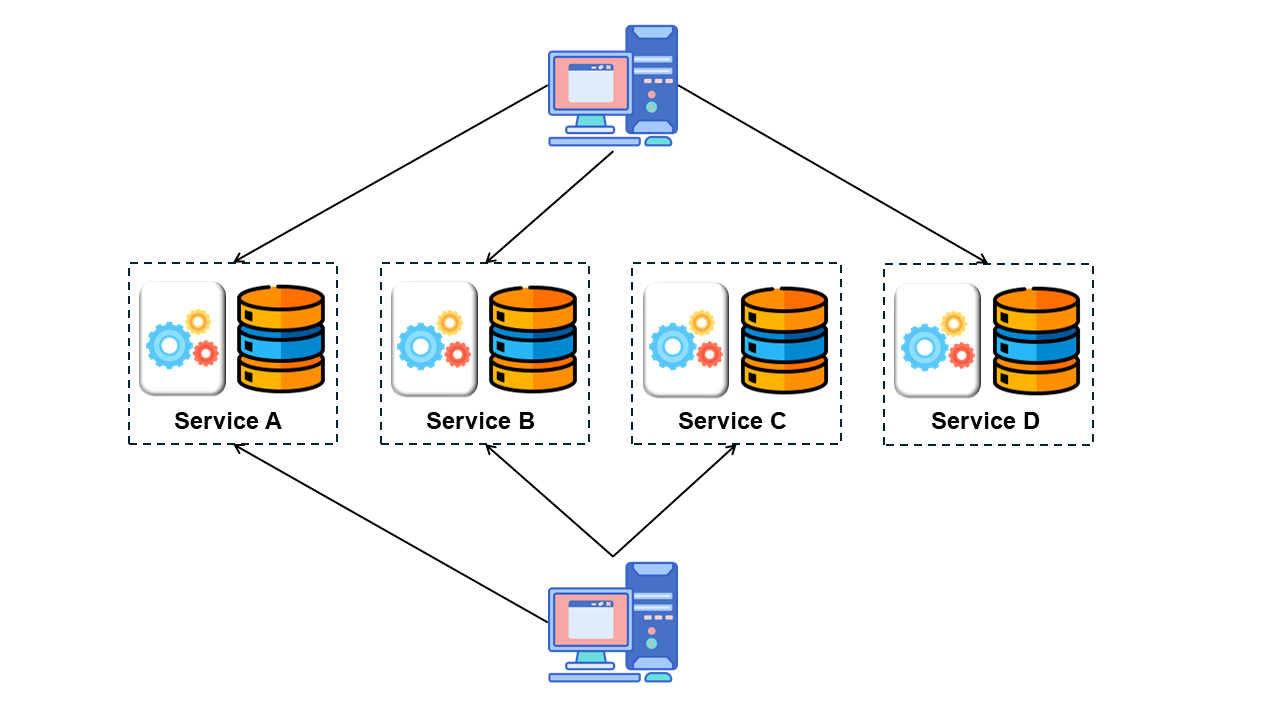
\includegraphics[trim=80 25 100 0,clip,height=0.98\paperheight]{diagrams/overview/soa}
    \end{adjustwidth}
	\begin{tikzpicture}[overlay,remember picture]
	\node[rectangle,shift={(1.8,3.6)},
		  text width=3cm,above] at (current page.west) {\color{primary}\Large SOA};
	\end{tikzpicture}   
\end{frame}
\note[itemize]{
    \item DB Icon made by setiawanap from www.flaticon.com
    \item Cogs Icon made by Design Circle from www.flaticon.com
}

\begin{frame}{SOA Circumvented}
    \begin{adjustwidth}{-10mm}{-10mm}
        \centering
        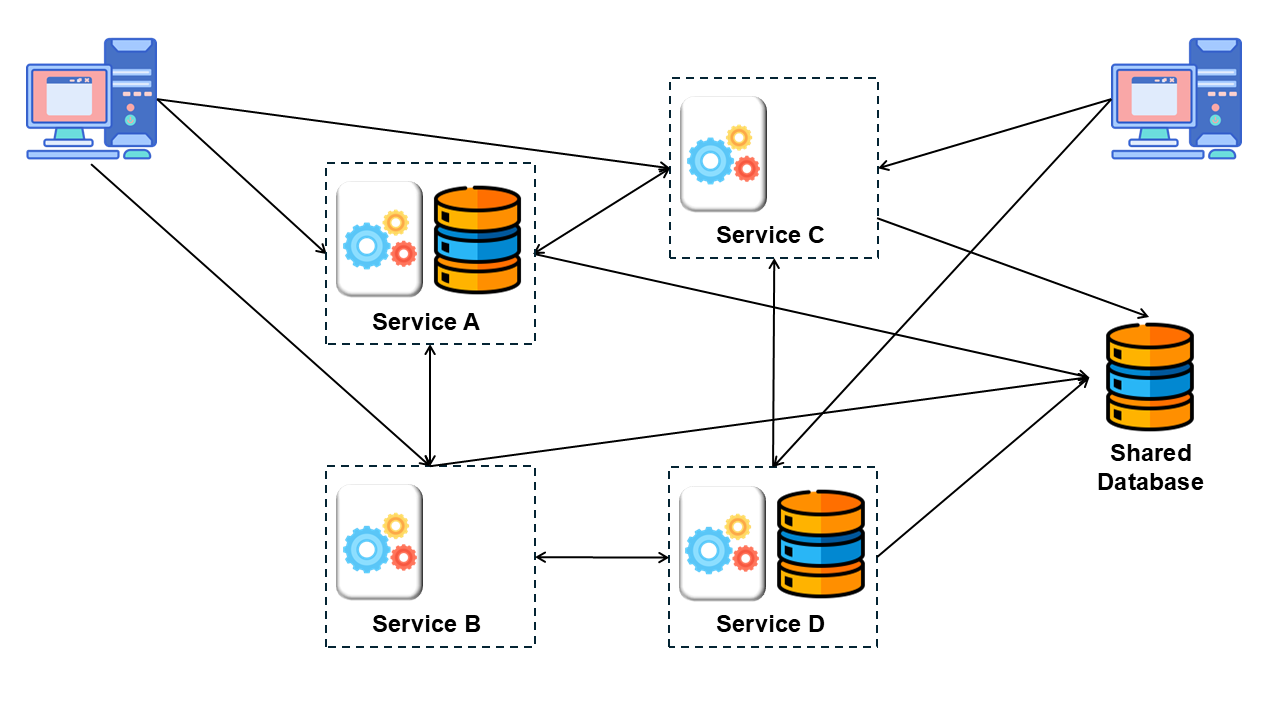
\includegraphics[trim=10 15 15 10,clip,width=0.98\paperwidth]{diagrams/overview/soa-circumvented}
    \end{adjustwidth}
\end{frame}

{
\usebackgroundtemplate{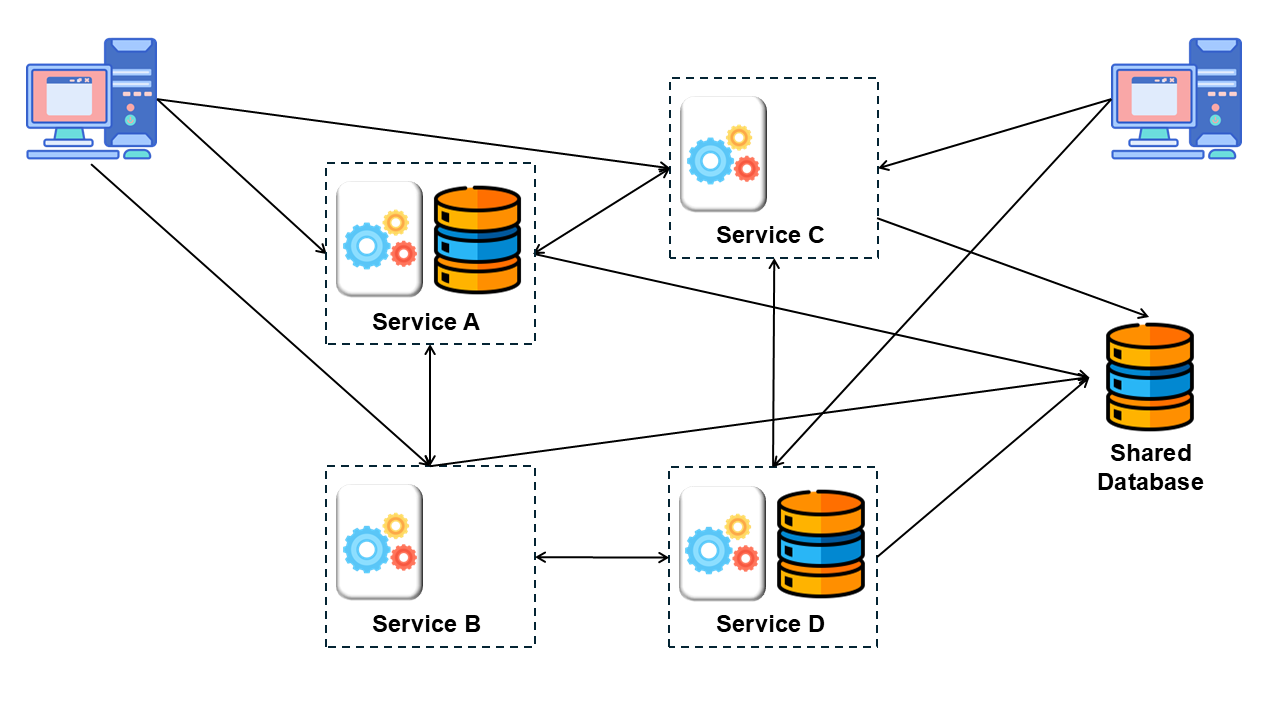
\includegraphics[trim=0 0 0 -41,clip,width=1.0055\paperwidth]{diagrams/overview/soa-circumvented}}
\begin{frame}{SOA Circumvented}
	\centering
	\includegraphics[height=.65\textheight]{../../shared/images/fear.png}
\end{frame}
}

\begin{frame}
    \begin{adjustwidth}{-10mm}{-10mm}
        \centering
        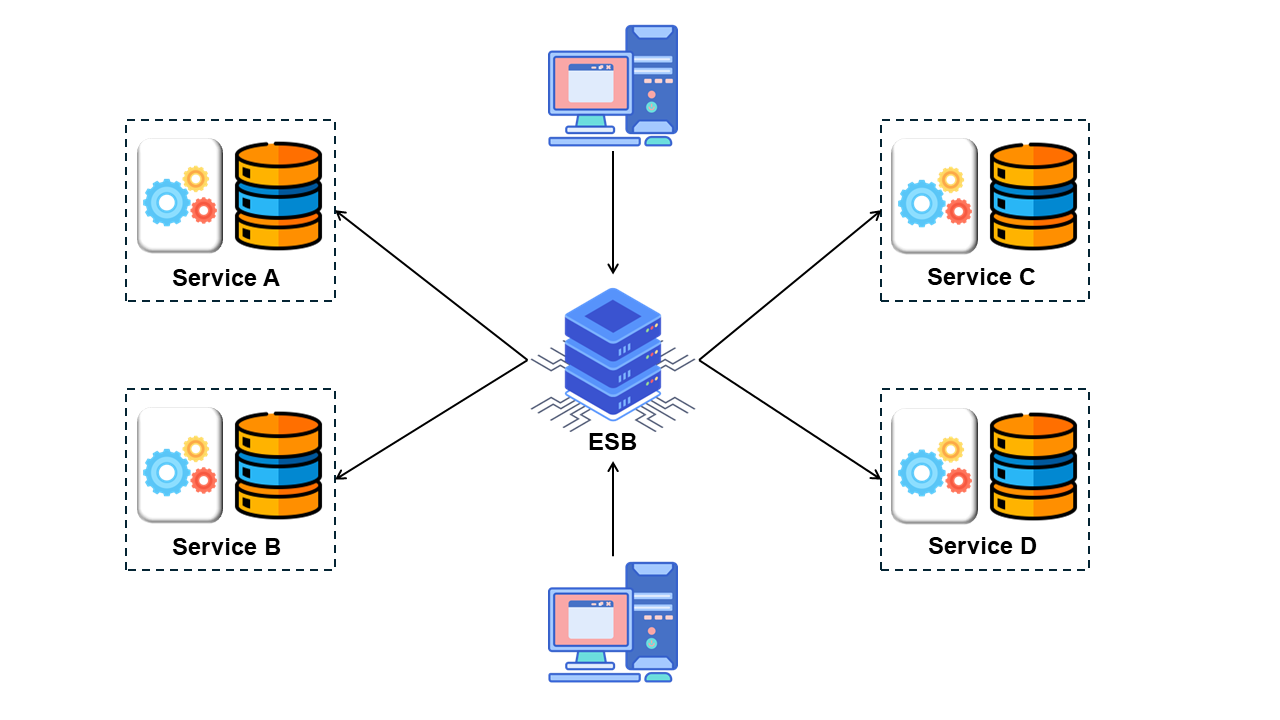
\includegraphics[trim=80 25 100 0,clip,height=0.98\paperheight]{diagrams/overview/esb}
    \end{adjustwidth}
	\begin{tikzpicture}[overlay,remember picture]
	\node[rectangle,shift={(1.8,3.6)},
		  text width=3cm,above] at (current page.west) {\color{primary}\Large ESB};
	\end{tikzpicture}   
\end{frame}
\note[itemize]{
    \item DB Icon made by setiawanap from www.flaticon.com
    \item Cogs Icon made by Design Circle from www.flaticon.com
    \item ESB Icon made by vectorsmarket15 from www.flaticon.com
}

\begin{frame}{ESB Circumvented}
    \begin{adjustwidth}{-10mm}{-10mm}
        \centering
        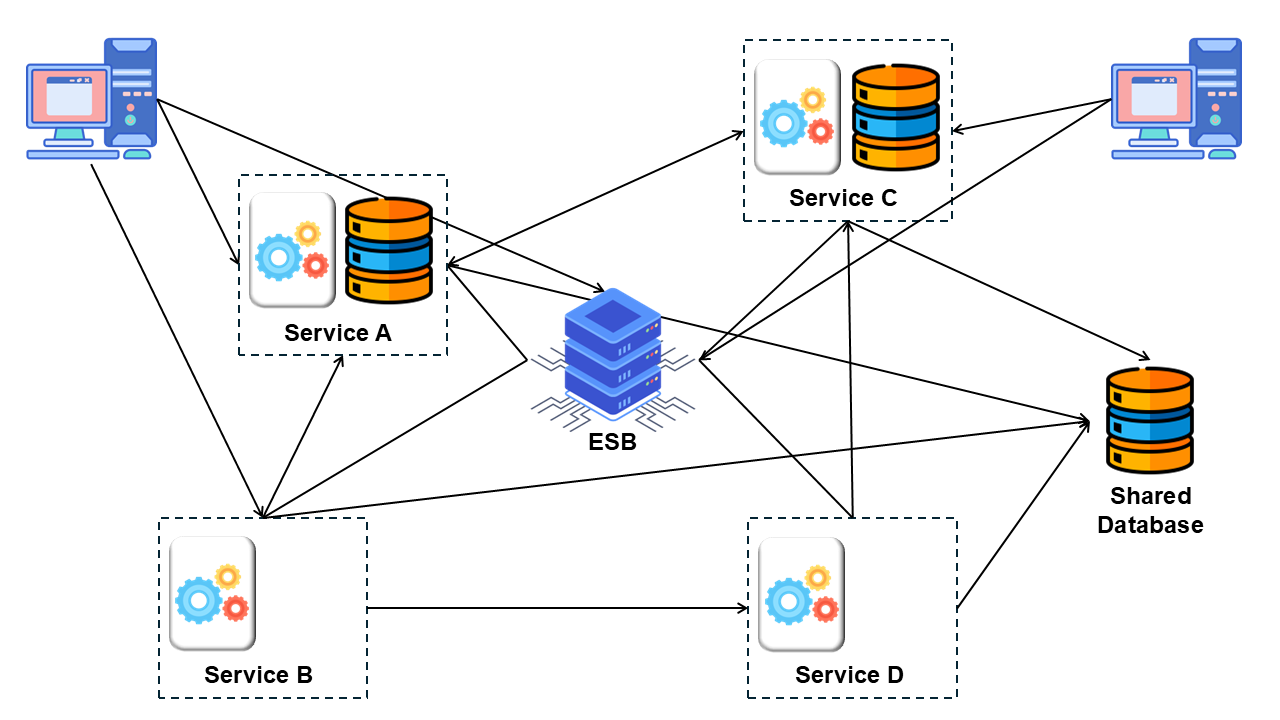
\includegraphics[trim=10 15 15 10,clip,width=0.9\paperwidth]{diagrams/overview/esb-circumvented}
    \end{adjustwidth}
\end{frame}

{
\usebackgroundtemplate{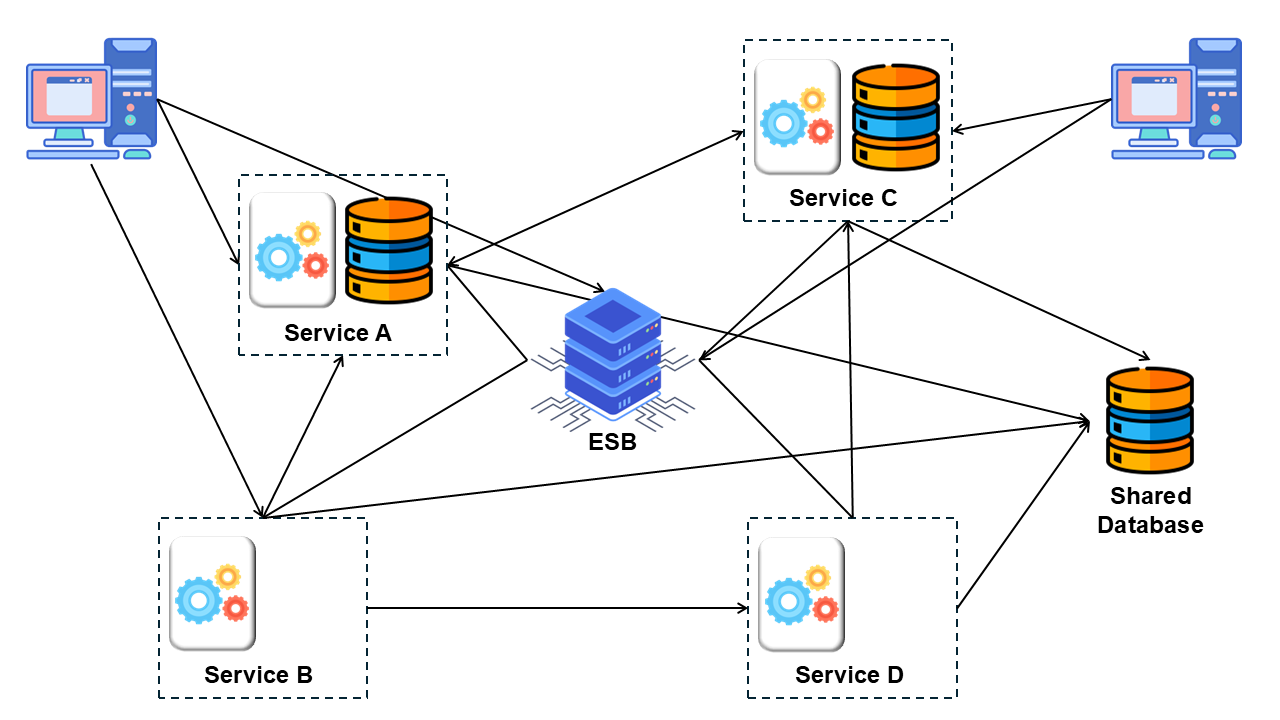
\includegraphics[trim=-42 0 0 -47,clip,width=0.965\paperwidth]{diagrams/overview/esb-circumvented}}
\begin{frame}{ESB Circumvented}
	\centering
	\includegraphics[height=.65\textheight]{../../shared/images/fear.png}
\end{frame}
}

\begin{frame}
    \begin{adjustwidth}{-10mm}{-10mm}
        \centering
        
\includegraphics[trim=80 25 100 0,clip,height=0.98\paperheight]{diagrams/overview/microservices}
    \end{adjustwidth}
	\begin{tikzpicture}[overlay,remember picture]
	\node[rectangle,shift={(3.4,3.6)},
		  text width=6cm,above] at (current page.west) {\color{primary}\Large REST-based Microservices};
	\end{tikzpicture}   
\end{frame}

\begin{frame}{REST-based Microservices Circumvented}
    \begin{adjustwidth}{-10mm}{-10mm}
        \centering
        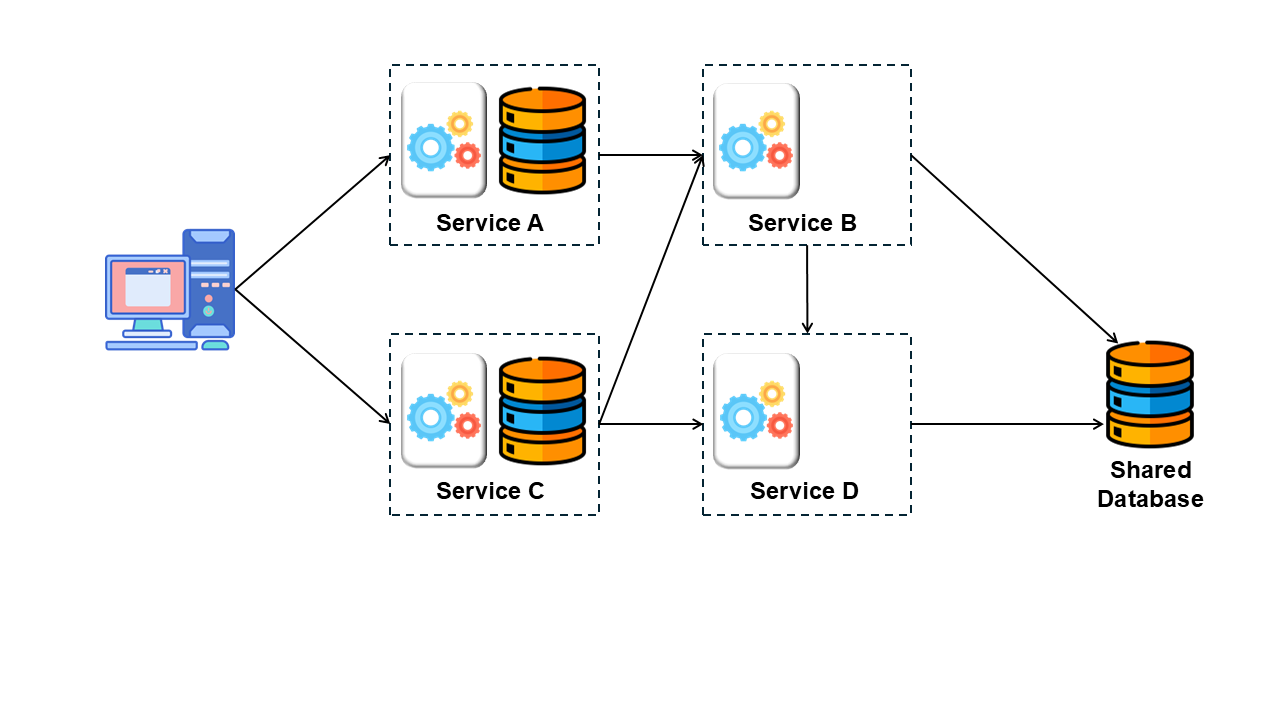
\includegraphics[trim=50 25 25 0,clip,width=\paperwidth]{diagrams/overview/microservices-circumvented}
    \end{adjustwidth}
\end{frame}

{
\usebackgroundtemplate{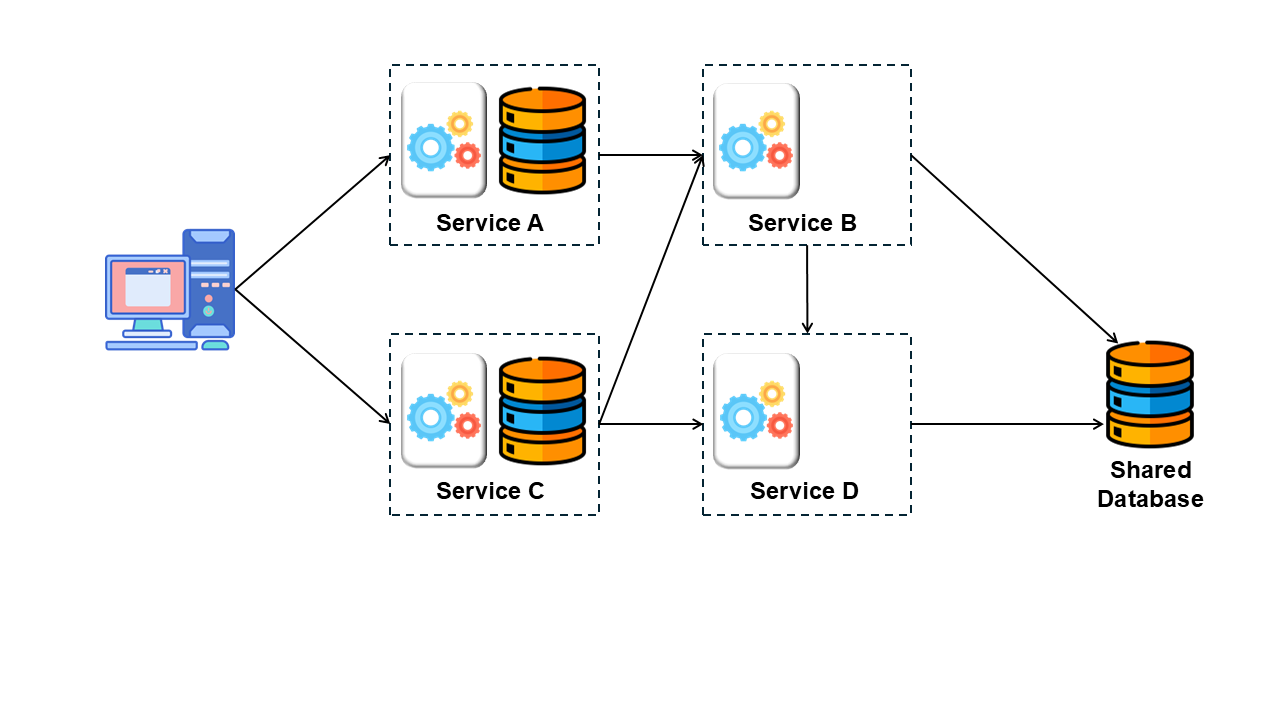
\includegraphics[trim=50 0 0 -47,clip,width=1.028\paperwidth]{diagrams/overview/microservices-circumvented}}
\begin{frame}{REST-based Microservices Circumvented}
	\centering
	\includegraphics[height=.65\textheight]{../../shared/images/fear.png}
\end{frame}
}

\questionanswer{Why does it go wrong?}{Getting caught up in the technology!}

\begin{frame}
    \centering
    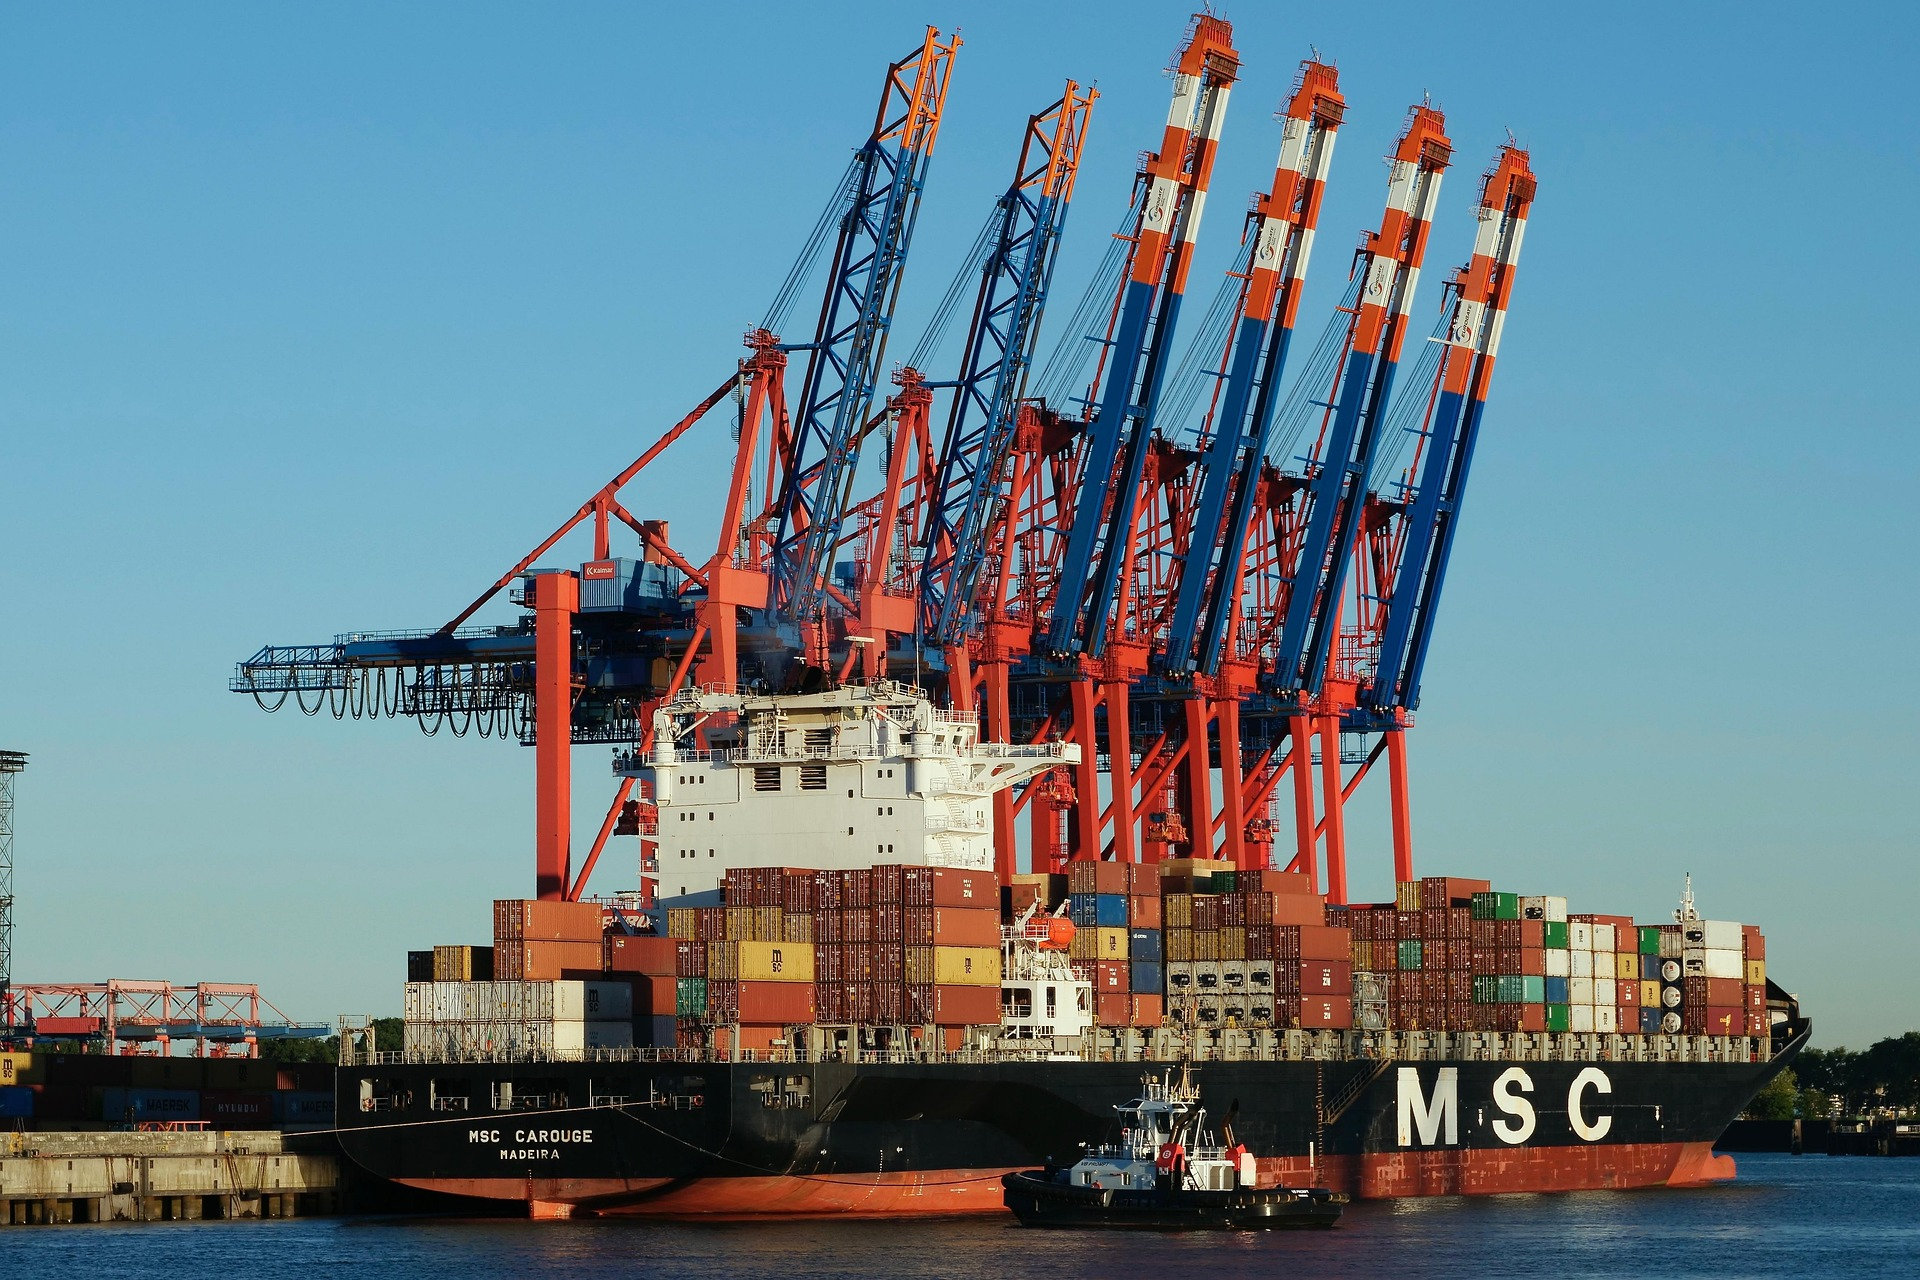
\includegraphics[width=0.62\paperwidth]{images/container-ship}\\
    \huge{
        If you haven't shipped \highlight{one} service.\\
        How will you ship a \highlight{dozen}?
    }
\end{frame}


\section{Microservices}

\begin{frame}{}
	\centering
	\includegraphics[trim=45 45 45 45,clip,height=\textheight]{diagrams/general-topology-deployment.png}
	\begin{tikzpicture}[overlay,remember picture]
	\node[rectangle,shift={(0.9,0.8)},
		  text width=7cm,above,rotate=90] at (current page.west) {\color{primary}\Large Microservices General Topology};
	\end{tikzpicture}   
\end{frame}
\note[itemize]{
    \item Multiple clients demonstrates common scenario of multiple interfaces to system (e.g. mobile, web).
    \item Client UIs may be monolithic to provide a rich interface.
}

\begin{frame}{API Layer Components}
    \centering
    \includegraphics[trim=45 45 45 45,clip,width=0.9\textwidth]{diagrams/general-topology-api-component.png}
\end{frame}
\note[itemize]{
    \item Each client may use a different combination of services.
    \item API layer provides reverse proxy or gateway services, see Service-Based Architecture notes \& slides.
    \item Typically Service APIs in this layer have a one-to-one relationship with Services and are designed by the Service teams.
    \item Routing behaviour may not be required.
}

\begin{frame}{Service 1 Components}
    \begin{adjustwidth}{-10.5mm}{-10mm}
        \centering
        \includegraphics[trim=45 45 45 45,clip,width=0.99\paperwidth]{diagrams/general-topology-service1-component.png}
    \end{adjustwidth}
\end{frame}
\note{Services 2 \& 3 are essentially the same.}

\begin{frame}{Client with Monolithic UI}
    \centering
    \includegraphics[trim=45 45 45 45,clip,width=0.9\textwidth]{diagrams/monolithic-ui-client1-component.png}
\end{frame}
\note[itemize]{
    \item Purist Microservices architecture -- each service development team builds their service's UI(s).
    \item Typically needs some coordinating activity in the UI.
    \item Can still have multiple UIs (e.g. web, mobile, ...).
}

\begin{frame}{Entity Service Anti-Pattern}
    \centering
    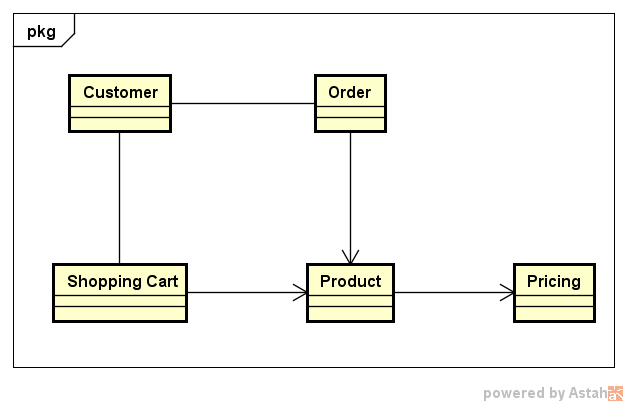
\includegraphics[trim=30 50 20 50,clip,width=0.8\paperwidth]{diagrams/esa-anti-pattern-classes}
\end{frame}
\note{
OO Modelling -- Identify entities in the problem domain
\begin{itemize}
    \item \large Tend to be stabler / longer-lived parts of the problem domain
\end{itemize}
}

\begin{frame}{Entity Service Anti-Pattern}
    \centering
    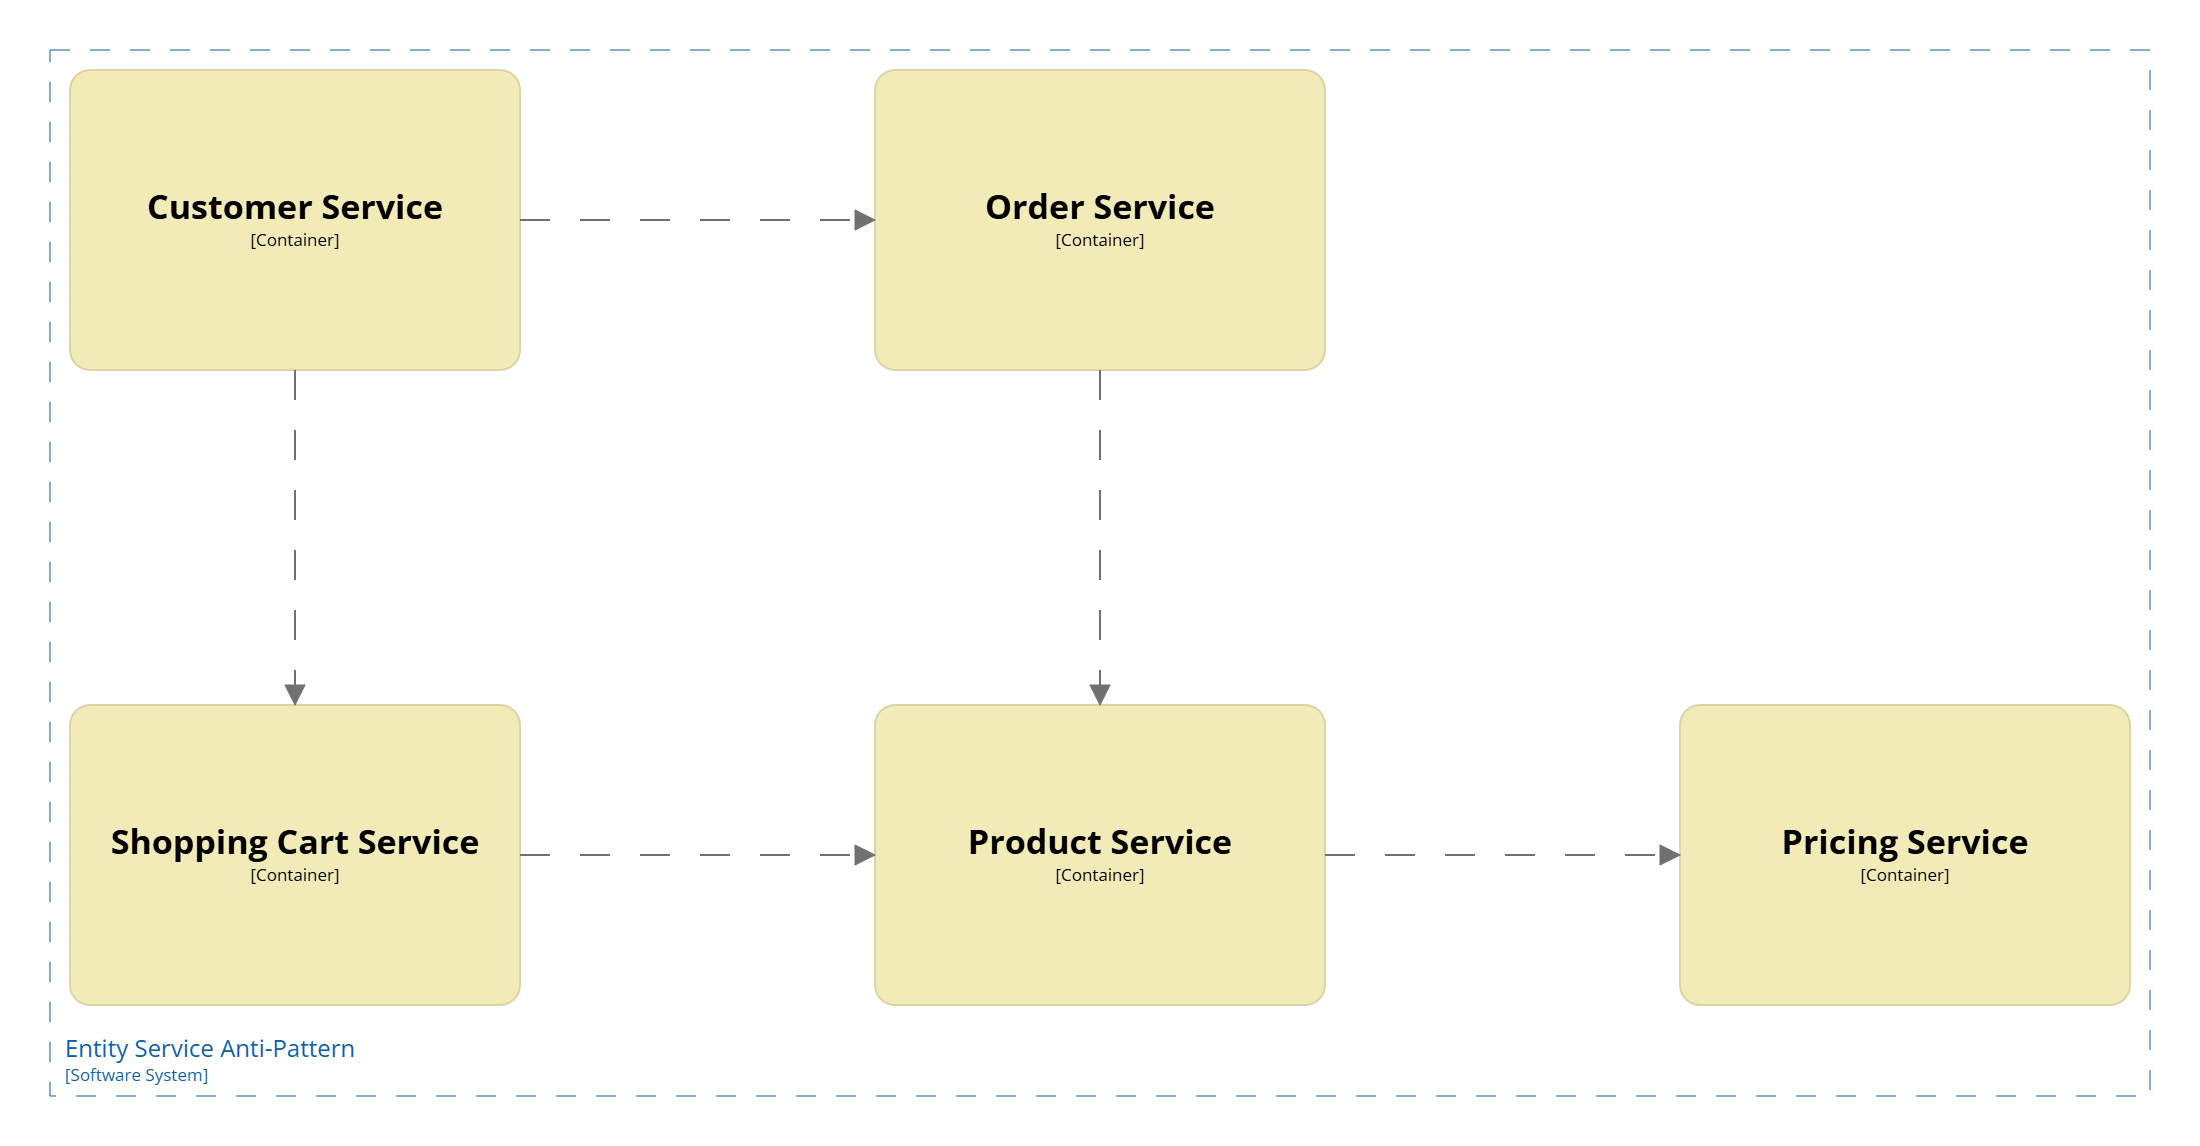
\includegraphics[trim=-25 5 5 5,clip,width=0.85\paperwidth]{diagrams/esa-anti-pattern}
\end{frame}
\note[itemize]{
    \item Intuitive approach -- Design services around main entities
    \item Usually introduces synchronous flow of logic between services
    \begin{enumerate}
        \item \large Customer places an Order
        \item \large Order calls Product to get details
        \item \large Product calls Pricing to determine price
    \end{enumerate}
}

\begin{frame}{Problem with Synchronous Logic}
    \vspace{1mm}
    \begin{columns}[t]
    \begin{column}{0.5\textwidth}
    {\LARGE
    \begin{itemize}
        \vspace{0.2em}
        \item Potential chain of failure
        \vspace{0.2em}
        \item Failures are multiplied
        \vspace{0.2em}
        \item Latency is multiplied
        \vspace{0.2em}
        \item Deployment is hard
        \vspace{0.2em}
        \item Scaling is hard
        \vspace{0.2em}
        \item Lazy design
    \end{itemize}
    }
    \end{column}
    \begin{column}{0.5\textwidth}
    {
    \centering
    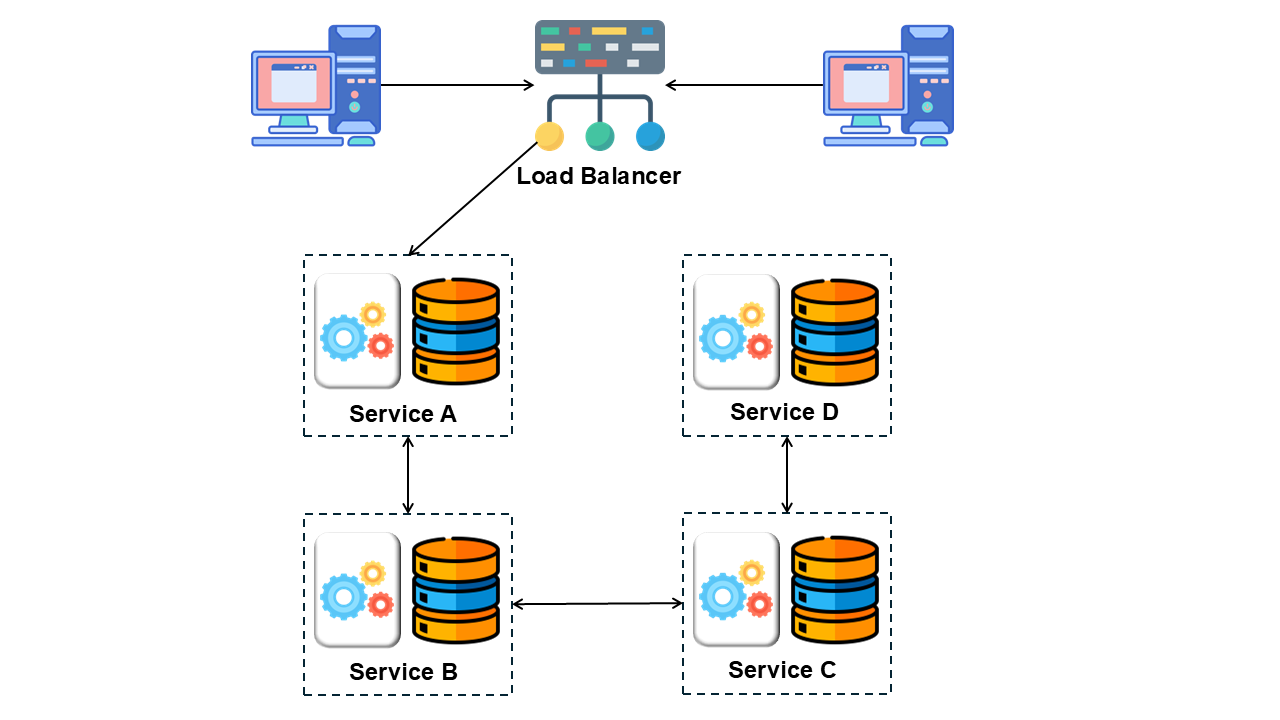
\includegraphics[trim=185 5 25 -20,clip,width=0.62\paperwidth]{diagrams/overview/synchronous}
    }
    \end{column}
    \end{columns}
	\begin{tikzpicture}[overlay,remember picture]
	\node[rectangle,shift={(-0.8,2.9)},
		  text width=3cm,above] at (current page.east) {
		      
\includegraphics[width=20mm]{images/tired}
		  };
	\end{tikzpicture}   
\end{frame}
\note[itemize]{
    \item DB Icon made by setiawanap from www.flaticon.com
    \item Cogs Icon made by Design Circle from www.flaticon.com
    \item Load Balancer Icon made by DinosoftLabs from www.flaticon.com
    \vspace{1em}
    \item Chains of request (synchronous logical flow) don't scale.
}


\section{Domain Driven Design}

\definition{Bounded Context}
{
    Logical boundary of a domain where particular terms and rules apply consistently.
}

\begin{frame}{}
	\centering
	\includegraphics[height=.97\textheight]{diagrams/bounded-context.png}
	\begin{tikzpicture}[overlay,remember picture]
	\node[rectangle,shift={(-4.6,0)},
		  text width=6.5cm,above] at (current page.south) {\color{primary}\tiny From \url{https://martinfowler.com/bliki/BoundedContext.html}};
	\end{tikzpicture}   
\end{frame}

\definition{Service Cohesion Principle}{
    Services are cohesive business processes.
}

\point[\Large DDD Consideration]{
    \vspace{0.5em}
    Services are \highlight{bounded contexts}.

    \vspace{0.5em}
    Bounded contexts are not necessarily \highlight{services}.
}

\point[\Large Large Bounded Contexts]{
    \vspace{0.5em}
    Bounded context may be too large to be a single service.

    \vspace{0.5em}
    Split it into services that are \highlight{independent} sub-processes.
}

\definition{Service Independence Principle}
{
    Services should not depend on the implementation of other services.
}

\corollary{Low Coupling}
{
    There should be minimal coupling between services.
}

\corollary{No Reuse}{
    Avoid dependencies between services.

    \vspace{0.3em}
    Do not reuse components between services.
}

\point[\Large Restaurant Examples]{
    \vspace{0.5em}
    Bad Restaurant

    \pause
    \vspace{0.5em}
    Good Restaurant
}

\point[\Large Lessons Learnt]{
    \vspace{0.5em}
    Chains of request don't \highlight{scale}.
    
    \vspace{0.5em}
    People who have the \highlight{information} to do their job are more effective.
    
    \vspace{0.5em}
    Service boundaries that follow these \highlight{principles} work better.
}

\point[\Large Human Shaped Microservices]{
    \vspace{0.5em}
    Look at \highlight{behaviour} rather than entities.
    \begin{itemize}
        \LARGE
        \item Who \& How
        \item Not the Thing
    \end{itemize}

    \vspace{0.5em}
    What would people \highlight{do}?

    \vspace{0.5em}
    How would they \highlight{communicate}?
}
\note{
    From Damian McLennan
}

\point[\Large Bounded Domains Implications]{
    \vspace{0.75em}
    \LARGE
    \begin{itemize}
		\item<1-> Duplication
	    \begin{itemize}
	    		\vspace{2mm}
			\Large\item Entities specialised for domain
		    \begin{itemize}
				\large\item Requires mapping of entity data between domains
		    \end{itemize}
	    		\vspace{2mm}
			\Large\item<2-> Should everything be duplicated?
		    \begin{itemize}
				\large\item<3-> What about common services (e.g. logging, ...)?
		    \end{itemize}
	    \end{itemize}
	    \vspace{3mm}
		\item<4-> Heterogeneity
		\begin{itemize}
	    		\vspace{1mm}
			\Large\item Services can use different implementation technologies
		\end{itemize}
    \end{itemize}
}

\section{Microservices Design Options}

\begin{frame}{Service Plane}
	\centering
	\includegraphics[height=.75\textheight]{diagrams/service-plane-sidecar.png}
	\begin{tikzpicture}[overlay,remember picture]
	\node[rectangle,shift={(-4.6,0)},
		  text width=6.5cm,above] at (current page.south) {\color{primary}\tiny From \textit{Fundamentals of Software Architecture}};
	\end{tikzpicture}   
\end{frame}

\begin{frame}{Service Mesh}
	\centering
	\includegraphics[height=.85\textheight]{diagrams/service-mesh.png}
	\begin{tikzpicture}[overlay,remember picture]
	\node[rectangle,shift={(-4.6,-0.1)},
		  text width=6.5cm,above] at (current page.south) {\color{primary}\tiny From \textit{Fundamentals of Software Architecture}};
	\end{tikzpicture}   
\end{frame}

{
\usebackgroundtemplate{\includegraphics[trim=-80 0 0 -35,clip,height=0.95\paperheight]{diagrams/service-mesh.png}}
\begin{frame}{Service Mesh}
	\centering
	\includegraphics[height=.65\textheight]{../../shared/images/fear.png}
	\begin{tikzpicture}[overlay,remember picture]
	\node[rectangle,shift={(-4.6,-0.1)},
		  text width=6.5cm,above] at (current page.south) {\color{primary}\tiny From \textit{Fundamentals of Software Architecture}};
	\end{tikzpicture}   
\end{frame}
}

\point[\Large Choreography \& Orchestration]{
\begin{description}
    \vspace{0.5em}
    \item[Choreography] Similar to event-driven \highlight{broker}
    \vspace{0.5em}
    \item[Orchestration] Similar to event-driven \highlight{mediator}
\end{description}
}

\begin{frame}
    \begin{adjustwidth}{-10mm}{-10mm}
        \centering
        \includegraphics[width=0.96\paperwidth]{diagrams/choreography.png}
    \end{adjustwidth}
	\begin{tikzpicture}[overlay,remember picture]
	\node[rectangle,shift={(1.7,3.6)},
		  text width=3cm,above] at (current page.west) {\color{primary}\Large Choreography};
	\end{tikzpicture}   
	\begin{tikzpicture}[overlay,remember picture]
	\node[rectangle,shift={(-4.7,-0.1)},
		  text width=6.5cm,above] at (current page.south) {\color{primary}\tiny From \textit{Fundamentals of Software Architecture}};
	\end{tikzpicture}   
\end{frame}

\begin{frame}
    \begin{adjustwidth}{-10mm}{-10mm}
        \centering
        \includegraphics[trim=-80 45 45 40,clip,width=0.89\paperwidth]{diagrams/sahara-choreography-deployment.png}
    \end{adjustwidth}
	\begin{tikzpicture}[overlay,remember picture]
	\node[rectangle,shift={(0.9,1.4)},
		  text width=6cm,above,rotate=90] at (current page.west) {\color{primary}\Large Sahara using Choreography};
	\end{tikzpicture}   
\end{frame}

\begin{frame}{}
    \begin{adjustwidth}{-10mm}{-10mm}
        \centering
        \includegraphics[trim=45 45 45 0,clip,width=0.98\paperwidth]{diagrams/sahara-choreography-purchase-products.png}
    \end{adjustwidth}
	\begin{tikzpicture}[overlay,remember picture]
	\node[rectangle,shift={(0.2,-0.9)},
		  text width=8cm,above] at (current page.north) {\color{primary}\Large Purchase Product Dynamic Diagram};
	\end{tikzpicture}   
\end{frame}

\begin{frame}
    \centering
    \includegraphics[height=.98\textheight]{diagrams/orchestration.png}
	\begin{tikzpicture}[overlay,remember picture]
	\node[rectangle,shift={(1.7,3.6)},
		  text width=3cm,above] at (current page.west) {\color{primary}\Large Orchestration};
	\end{tikzpicture}   
	\begin{tikzpicture}[overlay,remember picture]
	\node[rectangle,shift={(-4.6,0)},
		  text width=6.5cm,above] at (current page.south) {\color{primary}\tiny From \textit{Fundamentals of Software Architecture}};
	\end{tikzpicture}
\end{frame}

\questionanswer{How bad is coupling with choreography or orchestration?}
{For a large system, \highlight{very bad}.}
\note{In 2017, Uber had over 1400 services ... consider how bad coupling would be with either approach.}

\questionanswer{
    How do we scale large microservices-based systems?
}
{
    Combine architectural patterns
    \begin{itemize}
        \LARGE
        \item Event-Driven Microservices
    \end{itemize}
}

\begin{frame}{}
	\centering
	\includegraphics[trim=-50 45 45 45,clip,height=\textheight]{diagrams/event-queue-deployment.png}
	\begin{tikzpicture}[overlay,remember picture]
	\node[rectangle,shift={(0.9,0.8)},
		  text width=7cm,above,rotate=90] at (current page.west) {\color{primary}\Large Microservices with Event Queue};
	\end{tikzpicture}   
\end{frame}
\note[itemize]{
    \item Use the tried and true \highlight{Observer} pattern, with the \highlight{Event-Driven Architecture} pattern.
    \item Clients send \highlight{commands} telling services to do something
    \item Services \highlight{publish events} indicating what they have been done.
    \item Services \highlight{listen for events} to decide how to coordinate their part of the system behaviour.
}

\begin{frame}{Service 1 Components with Event Queue}
    \begin{adjustwidth}{-10.5mm}{-10mm}
        \centering
        \includegraphics[trim=45 45 45 45,clip,width=0.99\paperwidth]{diagrams/event-queue-service1-component.png}
    \end{adjustwidth}
\end{frame}
\note{Services 2 \& 3 are essentially the same.}

\begin{frame}{}
    \begin{adjustwidth}{-10.5mm}{-10mm}
		\centering
		\includegraphics[trim=-130 160 140 195,clip,height=\textheight]{diagrams/sahara-microservices-1-deploy.png}
    \end{adjustwidth}
	\begin{tikzpicture}[overlay,remember picture]
	\node[rectangle,shift={(0.9,1.4)},
		  text width=7cm,above,rotate=90] at (current page.west) {\color{primary}\Large Sahara using an Event Queue};
	\end{tikzpicture}   
\end{frame}
\note[itemize]{
    \item Sahara eCommerce system as a simple microservices architecture, using event-driven messaging between services.
    \item Services publish events indicating what they have been done.
    \item Also an example of a multi-tenanted system built across in-house servers, AWS and OCI.
}

\questionanswer{Are \highlight{browsing} and \highlight{purchasing} separate contexts?}{
\begin{itemize}
    \item Are they a single business process or different processes?
    \item Do they share much or little data?
\end{itemize}
}
\note[itemize]{
    \item Probably different business processes, but possibly the same context.
    \item If separate services, browse needs to send an event for every change to the shopping cart, and purchase needs to listen for these.
    \item Possibly merge into one service, as one context.
}

\question{
\begin{itemize}
    \item What about \highlight{inventory management} and \highlight{browse}?
    \item How do they maintain a consistent product database?
\end{itemize}
}

\point[\Large Model Behaviour]{
    \begin{itemize}
        \vspace{0.5em}
        \item \highlight{Commands} \& \highlight{Events} describe \highlight{behaviour}
        \vspace{0.5em}
        \item They will help you better model your \highlight{domain}
        \vspace{0.5em}
        \item Leading to \highlight{independent}, \highlight{scalable} services
    \end{itemize}
}

\begin{frame}{Pros \& Cons}
    \vspace{1mm}
    {\LARGE
    \begin{description}
        \item[Modularity] \tabto{15em}\includegraphics[width=8mm]{../../shared/images/thumbs-up.png}
        \item[Extensibility] \tabto{15em}\includegraphics[width=8mm]{../../shared/images/thumbs-up.png}
        \item[Reliability] \tabto{15em}\includegraphics[width=8mm]{../../shared/images/thumbs-up.png}
        \item[Interoperability] \tabto{15em}\includegraphics[width=8mm]{../../shared/images/thumbs-up.png}
        \item[Scalability] \tabto{15em}\includegraphics[width=8mm]{../../shared/images/thumbs-up.png}
        \item[Security] \tabto{15em}\includegraphics[trim=57 145 70 85,clip,width=8mm]{../../shared/images/neutral.png}
        \item[Deployability] \tabto{15em}\includegraphics[trim=22 19 22 12,clip,width=8mm]{../../shared/images/neutral.png}
        \item[Testability] \tabto{15em}\includegraphics[trim=22 19 22 12,clip,width=8mm]{../../shared/images/neutral.png}
        \item[Simplicity] \tabto{15em}\includegraphics[trim=22 19 22 12,clip,width=8mm]{../../shared/images/thumbs-down.png}
    \end{description}
    }
\end{frame}


%\bibliographystyle{ieeetr}
%\bibliography{books}

\end{document}